%!TEX root=../GaugeCNNTheory.tex


\subsection
    [Affine geometry of Euclidean spaces \texorpdfstring{$\Euc_d$}{}]%
    {Affine geometry of Euclidean spaces $\fakebold{\Euc}_{\boldsymbol{d}}$}
\label{sec:euclidean_geometry}


Before discussing coordinate free convolutions on Euclidean spaces, we need to understand the underlying Euclidean geometry.
Euclidean spaces $\Euc_d$ are by definition \emph{affine} spaces, that is, they come with an associated vector space of dimension $d$, which defines \emph{translations} on~$\Euc_d$.
In addition to being affine spaces, Euclidean spaces are endowed with an \emph{Euclidean metric} (distance function).
This distance functions corresponds to a Riemannian metric $\eta$, i.e. an $\O{d}$-structure $\OM$ on the (Riemannian) manifold $M=\Euc_d$.
This metric has the property that its curvature vanishes everywhere, that is, $\Euc_d$ is globally flat.


A standard example for Euclidean spaces are the \emph{vector spaces} $\R^d$, however, general Euclidean spaces consider less structure.
In particular, they do not come with a vector space structure and do thus not have a preferred origin.
Furthermore, they are in general not equipped with Cartesian coordinates.
We will therefore start with bare Euclidean spaces $\Euc_d$ and discuss how the relevant geometric structure is added to them.
One could in principle consider any $G$-structure, however, we are specifically interested in those $G$-structures that recover the classical steerable CNNs from the previous section, which explain all models in rows~(1-26) of Table~\ref{tab:network_instantiations}.
Such $\Aff(G)$-invariant $G$-structures are induced from $\Aff(G)$-atlases, consisting of charts of $\Euc_d$ whose transition functions take values in $\Aff(G)$ (Eq.~\eqref{eq:AffG_def}); see Fig.~\ref{fig:affine_charts}.
All statements made in coordinates $\R^d$ can via charts be translated to a coordinate free setting, which we develop here.
More infos about the relation between coordinate charts and gauges can be found in Appendix~\ref{apx:coordinate_bases}.

\begin{figure}
    \centering
    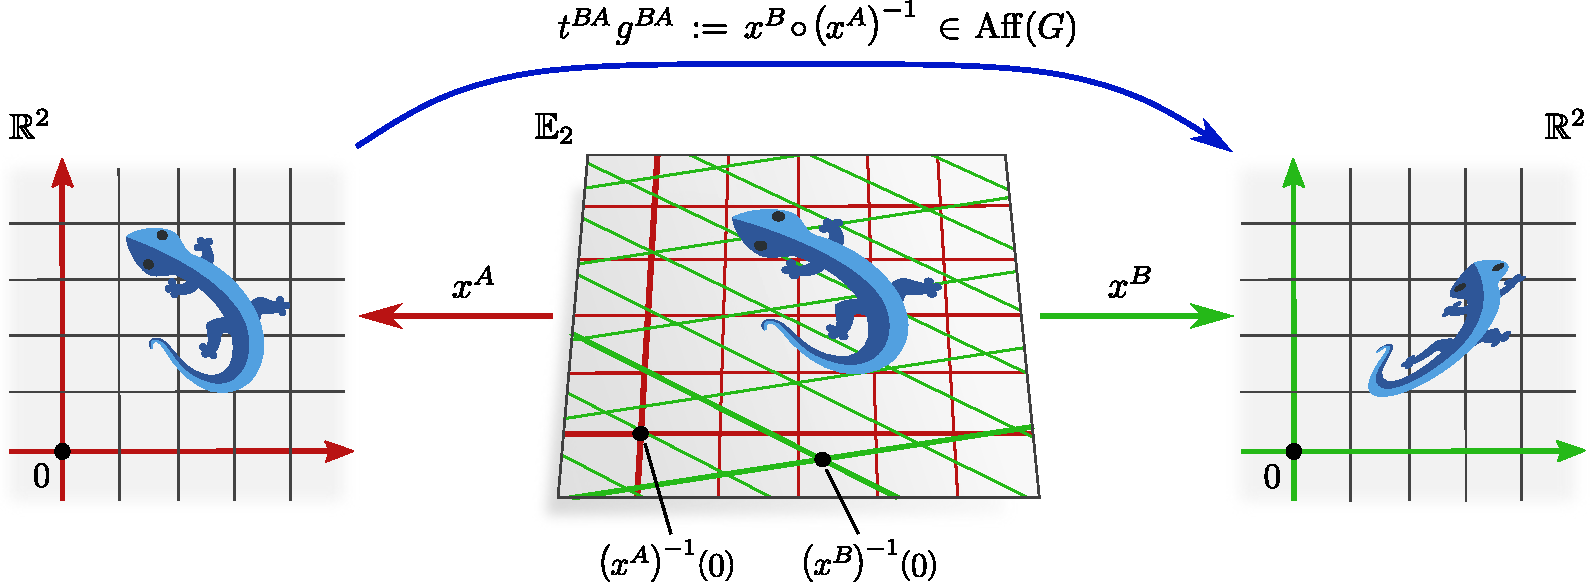
\includegraphics[width=1.\textwidth]{figures/affine_charts.pdf}
    \vspace*{2ex}
    \caption{\small
        Visualization of affine charts $x^X: \Euc_d \to \R^d$, which assign global coordinates to Euclidean spaces.
        Both $\Euc_d$ and $\R^d$ are affine spaces, such that one can demand the charts to be affine maps, which preserve collinearity and ratios of distances.
        We define an $\Aff(G)$-atlas $\mathscr{A}^{\Aff(G)}_{\Euc_d}$ as consisting of charts that are related by transition functions $t^{BA} g^{BA} := x^B \circ (x^A)^{-1}$ that are elements in $\Aff(G)$.
        Charts in an $\Aff(G)$-atlas differ at most in their choice of origin $(x^X)^{-1}(0)$ and a $G$-transformation.
        A choice of an $\Aff(G)$-atlas, consisting of charts $x^X$, induces a $G$-atlas $\mathscr{A}^G$ of gauges $\hat{d}x^X$.
        The corresponding $G$-structure $\GM$, which is in Fig.~\ref{fig:G_structures_R2_main} exemplified for different groups $G$, is invariant under the action of $\Aff(G)$.
        Theorem~\ref{thm:affine_equivariance_Euclidean_GM_conv} proves that $\GM$-convolutions on such $G$-structures are $\Aff(G)$-equivariant.
        {\\
        \color{gray}
        \scriptsize
            (Lizards adapted under the Creative Commons Attribution 4.0 International
            \href{https://github.com/twitter/twemoji/blob/gh-pages/LICENSE-GRAPHICS}{\underline{license}}
            by courtesy of Twitter.)
        }
    }
    \label{fig:affine_charts}
\end{figure}


\subsubsection{Affine charts and Aff(\textit{G})-atlases}
A Euclidean space $\Euc_d$ of dimension $d$ is homeomorphic to $\R^d$, and admits therefore global charts%
\footnote{
    The fact that $\Euc_d$ and $\R^d$ are globally homeomorphic (or even isometric) explains why most related work considers the vector spaces $\R^d$ as models of Euclidean spaces.
    Our approach in this section is a bit more careful as it introduces the minimal structure necessary to define $\GM$-coordinate independent convolutions on Euclidean spaces $M=\Euc_d$.
}
\begin{align}
    x^A: \Euc_d \to \R^d \,.
\end{align}
In the following we will always require these charts to be affine maps, i.e. isomorphisms of affine spaces, which preserve collinearity (i.e. they map straight lines to straight lines) and ratios of distances.
Since compositions of affine maps are affine maps, it follows that the chart transition functions
\begin{align}
    x^B \mkern-1mu\circ\mkern-1mu \big(x^A \big)^{-1}:\ \R^d \to \R^d
\end{align}
are affine transformations of $\R^d$, i.e. elements in $\Aff(\GL{d})$.
The transition functions decompose therefore uniquely into a translation $t^{BA} \in \Trans_d$ and an element $g^{BA} \in \GL{d}$:
\begin{align}
    t^{BA} g^{BA}\ :=\ x^B \mkern-1mu\circ\mkern-1mu \big(x^A \big)^{-1}
\end{align}
The notation $g^{BA}$ is hereby not accidental as these group elements agree with the gauge transformations that are induced by chart transitions, which is proven in Theorem~\ref{thm:AffG_atlas_induced_G_atlas} below.

Given a choice of affine group $\Aff(G)$, we define $\Aff(G)$-atlases of $\Euc_d$ as those atlases of global charts from $\Euc_d$ to $\R^d$, whose chart transition functions take values in $\Aff(G)$:
\begin{dfn}[$\Aff(G)$-atlas of Euclidean space]
\label{dfn:AffG_atlas}
    Let $\mathfrak{X}$ be an index set labeling charts and, for any ${X \mkern-2mu\in \mathfrak{X}}$, let $x^X: \Euc_d \to \R^d$ be a global affine chart of $\Euc_d$.
    The atlas
    \begin{align}
        \mathscr{A}^{\Aff(G)}_{\Euc_d}\ =\ \pig\{ \big( \Euc_d, x^X \big) \;\pig|\ X\in \mathfrak{X} \,\pig\}
    \end{align}
    is said to be an $\Aff(G)$-atlas if all of its chart transition functions take values in $\Aff(G)$, that is, if
    \begin{align}
        x^B \mkern-3mu\circ\mkern-2mu \big(x^A\big)^{-1} \!\in \Aff(G) \quad \forall\ A,B \in \mathfrak{X} \,.
    \end{align}
\end{dfn}
Fig.~\ref{fig:affine_charts} visualizes affine charts and the $\Aff(G)$-valued chart transition maps between them.


\subsubsection{Induced \textit{G}-atlases and \textit{G}-structures}
Any global coordinate chart $x^A: \Euc_d \to \R^d$ induces a global gauge, which is pointwise given by the chart gradients
\begin{align}
    \psiTMp^A := \hat{d}x_p^A :\ \TpM \to \R^d \,,
\end{align}
see Eq.~\eqref{eq:chart_differential_via_gradients} in Appendix~\ref{apx:chart_induced_bases_main} and Table~\ref{tab:coord_charts_gauge_trafos}.
An atlas of charts corresponds therefore an atlas of gauges.
In particular, given that the charts form an $\Aff(G)$-atlas, it is guaranteed that the gauge transformations are $G$-valued, that is, that the induced gauges form a $G$-atlas:
\begin{thm}[$\Aff(G)$-atlases of charts induce $G$-atlases of gauges]
\label{thm:AffG_atlas_induced_G_atlas}
    Let ${\mathscr{A}^{\Aff(G)}_{\Euc_d} \!= \big\{ ( \Euc_d, x^X ) \big| X \mkern-2mu\in\mkern-2mu \mathfrak{X} \big\}}$ be an $\Aff(G)$-atlas of \emph{charts}.
    The induced atlas of \emph{gauges}
    \begin{align}
        \mathscr{A}^G = \pig\{ \big(\Euc_d, \hat{d}x^X \big) \,\pig|\, X \in \mathfrak{X} \pig\}
    \end{align}
    is then guaranteed to be a $G$-atlas.
    In particular, if the chart transition maps are given by ${x^B \circ (x^A)^{-1}} = t^{BA} g^{BA}$, the transition maps between gauges are at any point $p\in \Euc_d$ given by ${g_p^{BA} = g^{BA} \in G}$.
\end{thm}
\begin{proof}
    The transition functions between chart induced gauges coincide by Eq.~\eqref{eq:chart_differential_trafo_law} with the Jacobian of the chart transition maps, that is,
    \begin{align}
        g_p^{BA} \,=\, \hat{d}x^B_p \circ \big(\hat{d}x^A_p \big)^{-1} \,=\, \frac{\partial x^B}{\partial x^A} \Big|_{x^A(p)} \,.
    \end{align}
    The last expression is the usual abuse of notation for Jacobians of chart transition maps, which was in Eq.~\eqref{eq:abuse_of_notation_jacobian} in components defined as
    \begin{align}
        \frac{\partial x^B_\mu}{\partial x^A_\nu} \bigg|_{x^A(p)}
        \,:=\,
        \partial_\nu \pig(x^B_\mu \circ \big(x^A\big)^{-1} \pig) \Big|_{x^A(p)} \,.
    \end{align}
    Using that the chart transition maps are given by $x^B \circ \big(x^A\big)^{-1} = t^{BA} g^{BA}$, this implies
    \begin{align}
        \big( g_p^{BA} \big)_{\mu\nu}
        \ =\ \partial_\nu \pig(x^B_\mu \circ \big(x^A\big)^{-1} \pig) (\mathscr{x}) \big|_{x^A(p)}
        \ =\ \partial_\nu \big( g^{BA} \mathscr{x} + t^{BA} \big)_\mu \big|_{x^A(p)}
        \ =\ g^{BA}_{\mu\nu} \,,
    \end{align}
    that is, that the induced gauge transformations $g_p^{BA}$ are $G$-valued and agree with $g^{BA}$ (which justifies the notation).
    As this argument holds for any $p\in \Euc_d$ and any charts $A,B \in \mathfrak{X}$, this implies that the induced atlas of gauges is a $G$-atlas.
\end{proof}


\begin{figure}
    \centering
    \begin{subfigure}[b]{0.46\textwidth}
        \centering
        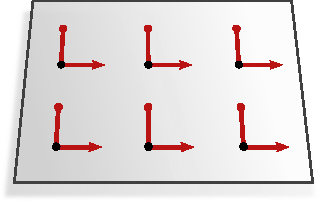
\includegraphics[width=.7\textwidth]{figures/G_structure_R2_1.pdf}
        \captionsetup{format=hang}
        \caption{\small
            $\Aff(\{e\})$-atlas induced $\{e\}$-structure $\eM$ on ${M=\Euc_2}$, preserved by \emph{translations} in $\Aff(\{e\}) = \IsomeM = \Trans_2$.
        }
        \label{fig:G_structure_R2_1}
    \end{subfigure}
    \hfill
    \begin{subfigure}[b]{0.46\textwidth}
        \centering
        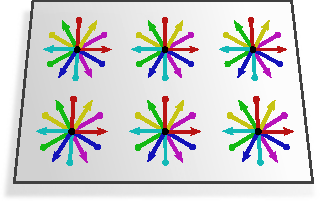
\includegraphics[width=.7\textwidth]{figures/G_structure_R2_2.pdf}
        \captionsetup{format=hang}
        \caption{\small
            $\Aff(\SO2)$-atlas induced $\SO2$-structure $\SOM$ on $M=\Euc_2$, preserved by \emph{translations} and \emph{rotations} in $\Aff(\SO2) = \IsomSOM = \SE2$.
        }
        \label{fig:G_structure_R2_2}
    \end{subfigure}
    \\[3ex]
    \begin{subfigure}[b]{0.46\textwidth}
        \centering
        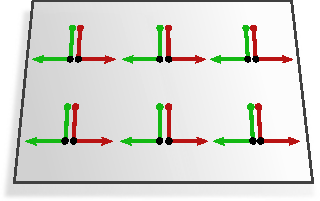
\includegraphics[width=.7\textwidth]{figures/G_structure_R2_3.pdf}
        \captionsetup{format=hang}
        \caption{\small
            $\Aff(\Flip)$-atlas induced $\Flip$-structure $\RM$ on $M=\Euc_2$, preserved by \emph{translations} and \emph{reflections} in $\Aff(\Flip) = \IsomRM = \Trans_2 \rtimes \Flip$.
            \\
        }
        \label{fig:G_structure_R2_3}
    \end{subfigure}
    \hfill
    \begin{subfigure}[b]{0.46\textwidth}
        \centering
        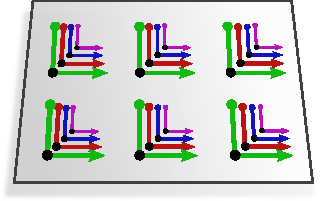
\includegraphics[width=.7\textwidth]{figures/G_structure_R2_4.pdf}
        \captionsetup{format=hang}
        \caption{\small
            $\Aff(\Scale)$-atlas induced $\Scale$-structure $\SM$ on $M=\Euc_2$, preserved by \emph{translations} and \emph{scalings} in $\Aff(\Scale) = \Trans_2 \rtimes \Scale$.
            Note that $\IsomSM = \Trans_2$ since scalings are non-isometric.
        }
        \label{fig:G_structure_R2_4}
    \end{subfigure}
    \vspace*{0ex}
    \caption{\small
        Visualization of different $G$-structures $\GM$ on Euclidean spaces $M=\Euc_2$ which are induced by an $\Aff(G)$-atlas of charts (Def.~\ref{dfn:AffG_atlas}).
        Fig.~\ref{fig:G_structure_R2_1} shows the translation invariant $\{e\}$-structure $\eM$ that corresponds to conventional Euclidean convolutions.
        The other three $G$-structures correspond to non-trivially $G$-steerable CNNs.
        They generalize locally over all poses that are related by the specific set of reference frames in $\GpM$.
        As the $G$-structures are $\Aff(G)$-invariant (implied by Theorem~\ref{thm:Aff_GM_in_charts}), the $G$-steerable convolutions are globally equivariant w.r.t. $\Aff(G)$ (Theorem~\ref{thm:affine_equivariance_Euclidean_GM_conv}).
        Instead of defining the $G$-structures via an $\Aff(G)$-atlas of charts, one could define them via a $G$-lift $\GM := \eM \lhd G$ of the canonical $\{e\}$-structure of $\R^d$ (Eq.~\eqref{eq:G_lifted_G_structure_Rd}), which augments the frames in the $\{e\}$-structure with all $G$-related frames.
     }
    \label{fig:G_structures_R2_main}
\end{figure} 


As discussed in Section~\ref{sec:bundle_trivializations}, any $G$-atlas of gauges implies a $G$-structure $\GM$.
According to Eq.~\eqref{eq:G_atlas_induced_G_structure_GM_def_ptwise}, $\GM$ is pointwise determined by
\begin{align}
    \GpM\ :=\ \big( \psiFMp^A \big)^{-1} (G) \,,
\end{align}
where the particular choice of gauge $A \in \mathfrak{X}$ is arbitrary.
The frames in $\GpM$ are the coordinate bases 
$\big[ \frac{\partial}{\partial x^A_\mu} \big|_p \big]_{\mu=1}^d = \big[\big(\hat{d}x_p^A \big)^{-1} (\epsilon_\mu) \big]_{\mu=1}^d$
and all $G$-transformations of them.
As the maximal $\Aff(G)$-atlas is by definition $\Aff(G)$-invariant, the same holds for the induced $G$-structure (with the action defined via any chart, as clarified and proven below).
Fig.~\ref{fig:G_structures_R2_main} shows such $G$-structures for different affine groups.
In the next section we prove that the corresponding $\GM$-convolutions are equivariant under the action of~$\Aff(G)$.


As it turns out, $\GM \xrightarrow{\piGM} \Euc_d$ is (non-canonically) isomorphic to $\Aff(G) \xrightarrow{\mathscr{q}} \Aff(G)/G \cong \R^d$ as a principal bundle, where
\begin{align}
    \mathscr{q}:\ \Aff(G) \to \R^d,\ \ tg \mapsto t
\end{align}
is the canonical quotient map of the affine group (after identifying cosets $tG$ with translations~$t$).%
\footnote{
    We implicitly employ a canonical isomorphism $\Aff(G)/G \xrightarrow{\sim} \R^d,\ \ tG \mapsto t$, where $t$ denotes a translation group element in $\Trans_d = (\R^d,+)$ on the l.h.s. and a vector in $\R^d$ on the r.h.s.
}
Non-surprisingly, this principal bundle isomorphism depends on the choice of chart.

\begin{thm}[Principal bundle isomorphism between Aff(\textit{G}) and \textit{GM}]
\label{thm:}
    Let $\GM$ be an $\Aff(G)$-atlas induced $G$-structure on $\Euc_d$.
    Then $\GM$ is isomorphic to $\Aff(G) \xrightarrow{\mathscr{q}} \R^d$ as a principal bundle, i.e. there are isomorphisms
    \begin{align}\label{eq:principal_bundle_iso_AffG_GM}
        \alpha^A: \Aff(G) \to \GM,\ \ tg \mapsto \big( \psiGMxAinvt \big)^{-1}(g)
    \end{align}
    and
    \begin{align}
        \big( x^A \big)^{-1}: \R^d \to \Euc_d
    \end{align}
    such that the following diagram commutes:
    \begin{equation}\label{cd:GM_def_embedding}
    \begin{tikzcd}[row sep=2.5em, column sep=7.em]
        \Aff(G) \times G
            \arrow[r, "\alpha^A \times \id_G"]
            \arrow[d, "\cdot\,"']
        & \GM \times G
            \arrow[d, "\,\lhd"]
        \\
        \Aff(G)
            \arrow[r, pos=.5, "\alpha^A"]
            \arrow[d, "\mathscr{q}\,"']
        & \GM
            \arrow[d, "\,\piGM"]
        \\
        \R^d
            \arrow[r, pos=.55, "(x^A)^{-1}"']
        & \Euc_d
    \end{tikzcd}
    \end{equation}
    The inverse of $\alpha^A$ is hereby given by
    \begin{align}
        \big(\alpha^A \big)^{-1}: \GM \to \Aff(G),\ \ [e_i]_{i=1}^d \mapsto tg
        \quad \textup{where}\ \ 
        \begin{cases}
            t = x^A \circ \piGM \big( [e_i]_{i=1}^d \big) \\[1ex]
            g = \psi_{\protect\scalebox{.6}{$G\!M,$}\protect\scalebox{.7}{$\piGM([e_i]_{i=1}^d)$}}^A \big( [e_i]_{i=1}^d \big)
        \end{cases}
    \end{align}
    Note that the isomorphisms are in one-to-one correspondence to the $\Aff(G)$-compatible charts of the considered atlas.
\end{thm}
\begin{proof}
    To prove the statement, we need to show that $\alpha^A$ and $(\alpha^A)^{-1}$ are indeed inverse to each other, that $\alpha^A$ is a bundle map over $(x^A)^{-1}$ and that $\alpha^A$ is right $G$-equivariant.
    That $(\alpha^A)^{-1}$ is both a well defined left and right inverse of $\alpha^A$ is easily checked by the reader.
    That $\alpha^A$ is a bundle map over $(x^A)^{-1}$ means that the bottom square of the diagram commutes.
    This is seen by observing that
    $(x^A)^{-1} \circ \mathscr{q} (tg) = (x^A)^{-1} (t)$ and
    $\piGM \circ \alpha^A (tg) = \piGM \circ \big(\psiGMxAinvt \big)^{-1}(g) = (x^A)^{-1} (t)$
    agree for any $tg \in \Aff(G)$.
    The commutativity of the upper square in the diagram, i.e. the right $G$-equivariance of $\alpha^A$, follows from the fact that
    $\alpha^A (tg \cdot \tilde{g}) = \big(\psiGMxAinvt \big)^{-1}(g \tilde{g}) = \big(\psiGMxAinvt \big)^{-1}(g) \lhd \tilde{g} = \alpha^A(tg) \lhd \tilde{g}$
    holds for any $tg\in \Aff(G)$ and any $\tilde{g} \in G$.
    The second step made use of the fact that $\psiGMxAinvt$ is right $G$-equivariant (Eq.~\eqref{eq:right_equivariance_GM}), which implies the equivariance of its inverse.
    Together, these properties show that $\alpha^A$ is a principal bundle isomorphism.
\end{proof}




\subsubsection{Coordinate free affine transformations}
As we want to prove the equivariance of $\GM$-convolutions under affine transformations in a coordinate free setting, we need to introduce groups of affine transformations of~$\Euc_d$, instead of $\R^d$ as above.
The charts will relate the coordinate free affine groups to the affine groups $\Aff(G)$ of~$\R^d$.

We start with the full group
\begin{align}\label{eq:AffE_def}
    \AffE\ :=\ \big\{ \phi: \Euc_d \to \Euc_d \,\big|\, \textup{$\phi$ is an affine transformation of $\Euc_d$} \big\}
\end{align}
of affine transformations of a Euclidean space $\Euc_d$.
It is easy to prove that $\AffE$ is isomorphic to $\Aff(\GL{d})$, with isomorphisms given by $\phi \mapsto x^A \phi\, (x^A)^{-1}$ for an arbitrary choice of chart $x^A$.
This statement is proven in a more general setting in Theorem~\ref{thm:Aff_GM_in_charts} below.

As in the case of isometries, we define subgroups $\AffGM \leq \AffE$ of $G$-structure preserving affine transformations:
\begin{dfn}[\textit{G}-structure preserving affine transformations]
\label{dfn:AffGM}
    Let $\GM$ be any $G$-structure on $\Euc_d$.
    We define the corresponding subgroup of $G$-structure preserving affine transformations as
    \begin{align}
        \AffGM\ :=\ \big\{ \phi \in \AffE 
        \,\big|\, \dphiFM \GpM = \GphipM\ \ \ \forall p \in \Euc_d \big\} 
        \,\ \leq\ \AffE \,.
    \end{align}
\end{dfn}
Compare this definition to that of $\IsomGM$ in Def.~\ref{dfn:IsomGM}.
As in the case of $\IsomGM$, the gauge transformations that are induced by affine transformations in $\AffGM$ are guaranteed to be $G$-valued.
This statement is formalized by the following theorem, which is essentially analogous to Theorem~\ref{thm:isom_GM_in_coords}:
\begin{thm}[$\AffGM$ in local trivializations]
\label{thm:Aff_GM_in_gauges}
    Let $\phi \in \AffE$ be any isometry of $M=\Euc_d$.
    Then the following three statements are equivalent:
    \begin{enumerate}
        \item $\phi$ is $G$-structure preserving, that is, $\phi \in \AffGM$.
        \item The affine transformation pullback $\psiFMp^{\widetilde{A}}\, \dphiFM^{-1}$ of any gauge $\psiFMp^{\widetilde{A}}$ of the $G$-atlas of $\FM$ that defines~$\GM$ is $G$-compatible with that $G$-atlas.
        \item
        The coordinate expression of $\dphiFM$ relative to any gauges $\psiFMp^{\widetilde{A}}$ and $\psiFMphip^A$ from the $G$-atlas of $\FM$ takes values in the structure group, that is,
        ${g_\phi^{A\widetilde{A}}(p)
           := \psiFMphip^A \,\dphiFM\, \big(\psiFMp^{\widetilde{A}} \big)^{-1}}
           = \hat{d}x^A_{\phi(p)} \,\dphiTM\, \big(\hat{d}x^{\widetilde{A}}_p \big)^{-1}$
        is $G$-valued.
    \end{enumerate}
\end{thm}
\begin{proof}
    The proof is analogous to that of Theorem~\ref{thm:isom_GM_in_coords}.
    More generally, the statement holds for arbitrary $G$-structure preserving \emph{diffeomorphisms}.
\end{proof}


Induced gauge transformations describe the transformation of the coordinate expressions of bundle elements, e.g. tangent or feature vector coefficients.
The action of the affine transformation $\phi$ on the manifold $\Euc_d$ itself can also be described in coordinates~$\R^d$.
This is achieved by a left and right multiplication of $\phi$ with any (affine) chart, which we can w.l.o.g. take to be equal at the source and target location since we are only considering global charts.
The resulting coordinate expression $t_\phi^{AA} g_\phi^{AA}$, defined by the following commutative diagram,
\begin{equation}\label{cd:AffGM_in_chart}
    \begin{tikzcd}[row sep=2.5em, column sep=5em]
        \R^d
            \arrow[rrr, rounded corners, to path={ 
                    |- node[below, pos=.75]{\small$t_\phi^{AA} \mkern1mu g_\phi^{AA}$} ([yshift=-3.ex, xshift=0ex]\tikztotarget.south)
                    -- ([xshift=0ex]\tikztotarget.south)
                    }]
        &
        \Euc_d
            \arrow[l, "x^A"']
            \arrow[r, "\phi"]
        &
        \Euc_d
            \arrow[r, "x^A"]
        &
        \R^c
    \end{tikzcd}
\end{equation}
is guaranteed to take values in $\Aff(G)$ if $\phi$ preserves the $G$-structure.
\begin{thm}[$\AffGM$ in global affine charts]
\label{thm:Aff_GM_in_charts}
    Let $\GM$ be the $G$-structure induced by some $\Aff(G)$-atlas and let $x^A: \Euc_d \to \R^d$ be a chart of this atlas.
    The coordinate expression of an element $\phi \in \AffGM$ relative to $x^A$ is then given by
    \begin{align}\label{eq:AffGM_in_charts_eq}
        x^A \phi\, \big(x^A)^{-1} \,=:\, t_\phi^{AA} \mkern1mu g_\phi^{AA} \ \in\, \Aff(G) \ ,
    \end{align}
    where
    \begin{align}
        t_\phi^{AA} := x^A \,\phi\, \big(x^A \big)^{-1} (0) \ \in\ \Trans_d
        \qquad \textup{and} \qquad
        g_\phi^{AA} := 
        \hat{d}x^A_{\phi(p)} \,\dphiTM\, \big(\hat{d}x^A_p \big)^{-1} \ \in\ G
    \end{align}
    The element $g_\phi^{AA} \in G$ in the coordinate expression coincides hereby with the induced gauge transformation $g_\phi^{AA}(p) \in G$ from Theorem~\ref{thm:Aff_GM_in_gauges} at \emph{any} point $p \in \Euc_d$.

    Furthermore, the coordinatization map
    \begin{align}
        \AffGM \to \Aff(G),\,\ \ \phi \mapsto x^A \,\phi\, \big(x^A \big)^{-1} \,,
    \end{align}
    is a group isomorphism.
\end{thm}
\begin{proof}
    Since $x^A$ and $\phi$ are affine maps, $x^A \,\phi\, \big(x^A)^{-1}: \R^d \to \R^d$ is an affine transformation of $\R^d$, i.e. an element of $\Aff(\GL{d})$ (or some subgroup of it).
    This implies that a first order Taylor expansion of the expression is \emph{exact}.
    The application of the coordinate expression to an arbitrary element $\mathscr{x} \in \R^d$ can therefore be written in terms of the following Taylor expansion around the origin $0$ of $\R^d$:
    \begin{align}
        \big[ x^A \,\phi\, \big(x^A)^{-1} \big] (\mathscr{x})
        \ =&\ \big[ x^A \,\phi\, \big(x^A)^{-1} \big] (0)\ +\ 
            \frac{\partial}{\partial \mathscr{x}'} \big[ x^A \,\phi\, \big(x^A)^{-1} \big]_{\mathscr{x}' = 0} \cdot \mathscr{x} \notag \\
        \ =&\ t_\phi^{AA}\ +\ g_\phi^{AA} \cdot \mathscr{x} \notag \\
        \ =&\ \big( t_\phi^{AA} \mkern2mu g_\phi^{AA} \big) \, \mathscr{x}
    \end{align}
    Here we implicitly defined the translation $t_\phi^{AA} \in \R^d$ and the Jacobian $g_\phi^{AA} \in \R^{d\times d}$ and identified them with group elements, which is possible since all involved morphisms are invertible.

    That the Jacobian $g_\phi^{AA}$ agrees with the induced gauge transformation $g_\phi^{AA}(p)$ at an arbitrary point $p\in M$ is shown by rewriting it via Eq.~\eqref{cd:jacobian_def} in terms of differentials:
    \begin{align}
        g_\phi^{AA}
        \ &=\ \frac{\partial}{\partial \mathscr{x}'} \big[ x^A \,\phi\, \big(x^A)^{-1} \big]_{\mathscr{x}' = x^A(p)} \notag \\
        \ &=\ \iota_{\R^d}\, d\big[ x^A \,\phi\, \big(x^A)^{-1} \big]_{x^A(p)} \, \big(\iota_{\R^d} \big)^{-1} \notag \\
        \ &=\ \iota_{\R^d}\, dx^A_{\phi(p)} \,d\phi_p\, \big(dx^A_p)^{-1}\, \big(\iota_{\R^d} \big)^{-1} \notag \\
        \ &=\ \hat{d}x^A_{\phi(p)} \,\dphiTM\, \big(\hat{d}x^A_p)^{-1} \notag \\
        \ &=\ g_\phi^{AA}(p)
    \end{align}
    In the penultimate step we identified the differential $d\phi$ as an alternative notation for the pushforward $\dphiTM$ and identified the chart gradients $\hat{d}x^A := \iota_{\R^d}\, dx^A$ as defined in Eq.~\eqref{eq:chart_differential_via_gradients}.
    The index $p$ is dropped in the notation $g_\phi^{AA} = g_\phi^{AA}(p)$ due to its arbitrariness.

    That $t_\phi^{AA} g_\phi^{AA}$ is not only an element element of $\Aff(\GL{d})$ but of its subgroup $\Aff(G)$ is clear since Theorem~\ref{thm:Aff_GM_in_gauges} states that $g_\phi^{AA}(p) \in G$ for any $\phi \in \AffGM$.

    To prove that the coordinatization map $C^A: \AffGM \to \Aff(G),\,\ \phi \mapsto x^A \,\phi\, (x^A)^{-1}$ is indeed a group isomorphism, we need to show that it is
    1) a group homomorphism,
    2) injective and
    3) surjective.
    That $C^A$ is a group homomorphism follows immediately from its definition since
    \begin{align}
        C^A(\phi\, \tilde{\phi})
        \ =\ x^A\, \phi\, \tilde{\phi}\, \big(x^A\big)^{-1}
        \ =\ x^A\, \phi\, \big(x^A\big)^{-1}\, x^A\, \tilde{\phi}\, \big(x^A\big)^{-1}
        \ =\ C^A(\phi)\, C^A(\tilde{\phi})
    \end{align}
    holds for any $\phi,\tilde{\phi} \in \AffGM$.
    The injectivity of $C^A$ requires that, for any $\phi,\tilde{\phi} \in \AffGM$, the equality $C^A(\phi) = C^A(\tilde{\phi})$ implies $\phi = \tilde{\phi}$.
    That this is the case is clear since $C^A(\phi) = C^A(\tilde{\phi})$ is equivalent to 
    $x^A\, \phi\, \big(x^A\big)^{-1} = x^A\, \tilde{\phi}\, \big(x^A\big)^{-1}$, which implies the equality of $\phi$ and $\tilde{\phi}$ since $x^A$ is an isomorphism.
    Lastly, $C^A$ is surjective if and only if for any $tg \in \Aff(G)$ there exists some $\phi \in \AffGM$, such that $C^A(\phi) = tg$.
    As an ansatz, let $\phi = \big(x^A\big)^{-1} \,tg\, x^A$, such that $C^A(\phi) = tg$.
    What remains to be shown is that this construction of $\phi$ is indeed an element of $\AffGM$.
    As one can easily check, $g_\phi^{AA} = g \in G$, such that $\phi \in \AffGM$ follows from Theorem~\ref{thm:Aff_GM_in_gauges}, with which surjectivity holds.
    Overall, this proves that $C^A: \AffGM \to \Aff(G)$ is a group isomorphism if $\AffGM$ is induced by an $\Aff(G)$-atlas.
\end{proof}

The isomorphism between $\AffGM$ and $\Aff(G)$ is not unique, as it depends on the particular chart considered.
Different choices are related by the inner automorphisms of $\Aff(G)$ since
\begin{align}
    C^B(\phi) 
    = x^B \,\phi\, (x^B)^{-1}
    = x^B (x^A)^{-1} x^A \,\phi\, (x^A)^{-1} x^A (x^B)^{-1}
    = (t^{BA} g^{BA}) \,C^A(\phi)\, (t^{BA} g^{BA})^{-1}
    \,.
\end{align}
This concludes our analysis of the Euclidean geometry and $\Aff(G)$-invariant $G$-structures that are required for the definition of coordinate free Euclidean convolutions in the next section.
